\documentclass{article}
\usepackage[UTF8]{ctex}
\usepackage{amsmath}
\usepackage{amssymb}
\usepackage{tikz}
\usepackage{xcolor}
\usetikzlibrary{arrows,shapes,chains}
\usepackage{cite}
\usepackage{graphicx}
\usepackage{subfigure}
\usepackage{listings}
\usepackage{float}
%\usepackage[framed,numbered,autolinebreaks,useliterate]{mcode}

\title{Code2 实验报告}
\author{郑涛 SA24001077}
\date{\today}

\begin{document}
	\maketitle
	\section{问题描述}
	本次实验目的是实现$de\,Casteljau$算法和基于Bézier基函数的Bézier插值曲线,并具有交互功能。
	\section{程序思路说明}
	给定插值点$p_i(x_i,y_i)(i=0,1,\cdots,n)$
	\subsection{$de\,Casteljau$算法}
	对于任意的$t\in [0,1]$根据如下关系求出$x(t)=b_0^n$:
	$$b_i^k=tb_{i+1}^{k-1}+(1-t)b_i^{k-1}$$
	
	
	
\subsection{基于Bézier基函数插值算法}
	固定点$p_{i}(i=0,1,\dotsb,n)$,Bézier曲线上的点$x(t)$为所有固定点的一个插值,在$t(t \in [0,1])$时刻的$x(t)$有如下公式:
	$$x(t) = \sum\limits_{i=0}^{n}C_{n}^{i}B_{i}^{n}(t)p_{i}$$
	其中Bézier基函数:
	$$B_{i}^{n}(t)=t^{i}(1-t)^{n-i}$$
	

	\section{编译环境}
	本代码用MATLAB R2022b编译
	\section{使用说明}
	本代码可直接运行
	\section{主要代码展示}
	\lstset{language=Matlab}
	\lstset{breaklines}%自动将长代码换行排版
	\begin{lstlisting}
function p = bezier(p, t, h)
  p = p*[1;1i];
  x = zeros(1,length(t));
  n=length(p)-1;
  for i = 1:length(t)
    for j = 1:n+1
      x(i) = x(i) + factorial (n)/(factorial (n-j+1)*factorial (j-1))*t(i)^(j-1)*(1-t(i))^(n-j+1)*p(j);
    end
  end
  p=x;
  if nargin>2,set(h, 'xdata', real(p), 'ydata', imag(p)); end
end
function p = bezier_caste(p, t, h)
  p = p*[1;1i];
  x = zeros(1,length(t));
  n=length(p);
  for i = 1:length(t)
    b=p;
    for j = 1:n-1
      for k = n:-1:j+1
        b(k) = t(i)*b(k)+(1-t(i))*b(k-1);
      end
    end
    x(i)=b(n);
  end
  p=x;
  if nargin>2,set(h, 'xdata', real(p), 'ydata', imag(p)); end
end
	\end{lstlisting}
	\section{结果展示}
\begin{figure}[H]
	\centering
	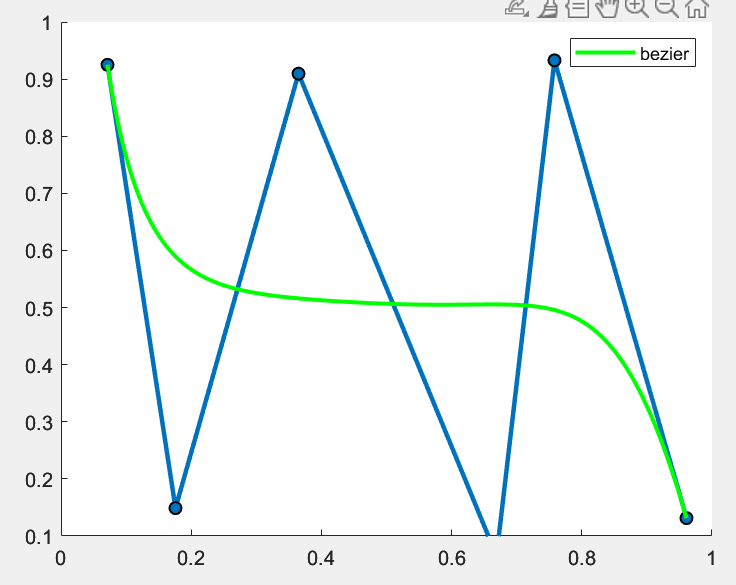
\includegraphics{bezier}
	\caption{基于Bézier基函数的Bézier插值曲线}
	\label{fig:bezier}
\end{figure}
\begin{figure}[H]
	\centering
	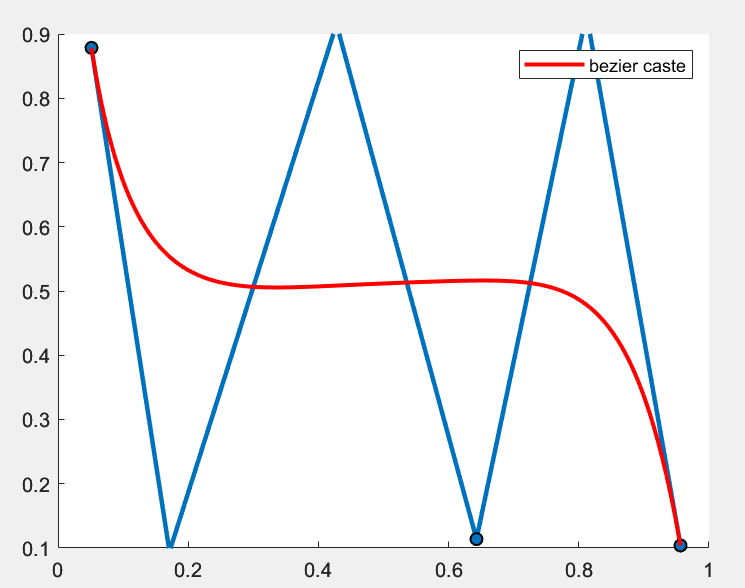
\includegraphics{bezier_caste}
	\caption{$de\,Casteljau$算法的Bézier插值曲线}
	\label{fig:bezier_caste}
\end{figure}


	\section{实验结果分析}
	完成了两个算法的Bézier插值并实现交互。
\end{document}